\documentclass[11pt,compress,t,notes=noshow, aspectratio=169, xcolor=table]{beamer}

\usepackage{../../style/lmu-lecture}
% Defines macros and environments
% This file is included in slides and exercises

% Rarely used fontstyle for R packages, used only in 
% - forests/slides-forests-benchmark.tex
% - exercises/single-exercises/methods_l_1.Rnw
% - slides/cart/attic/slides_extra_trees.Rnw
\newcommand{\pkg}[1]{{\fontseries{b}\selectfont #1}}

% Spacing helpers, used often (mostly in exercises for \dlz)
\newcommand{\lz}{\vspace{0.5cm}} % vertical space (used often in slides)
\newcommand{\dlz}{\vspace{1cm}}  % double vertical space (used often in exercises, never in slides)
\newcommand{\oneliner}[1] % Oneliner for important statements, used e.g. in iml, algods
{\begin{block}{}\begin{center}\begin{Large}#1\end{Large}\end{center}\end{block}}

% Don't know if this is used or needed, remove?
% textcolor that works in mathmode
% https://tex.stackexchange.com/a/261480
% Used e.g. in forests/slides-forests-bagging.tex
% [...] \textcolor{blue}{\tfrac{1}{M}\sum^M_{m} [...]
% \makeatletter
% \renewcommand*{\@textcolor}[3]{%
%   \protect\leavevmode
%   \begingroup
%     \color#1{#2}#3%
%   \endgroup
% }
% \makeatother


\title{Interpretable Machine Learning}
% \author{LMU}
%\institute{\href{https://compstat-lmu.github.io/lecture_iml/}{compstat-lmu.github.io/lecture\_iml}}
\date{}

\begin{document}

\newcommand{\titlefigure}{figure/pdp_bike}
\newcommand{\learninggoals}{
\item Understand c-ICE curves to identify the heterogeneity in the model
%\item Understand the usefullness of ICE curves and d-ICE curves in case of interaction effects
\item Understand the extrapolation issue}

\lecturechapter{Issues and Extensions of ICE and PD Plots}
\lecture{Interpretable Machine Learning}


\begin{frame}{Centered ICE Plot (c-ICE)}

\textbf{Issue:} Difficult to identify heterogenous ICE curves if curves have different intercepts (are stacked)
%When ICE curves start at different intercepts (are stacked), it is difficult to identify heterogenous predictions.

\textbf{Solution:} Center ICE curves at fixed reference value $x^* \sim \P(\xv_S)$, often $x^* = \min(\xv_S)$

\begin{columns}[c]
\begin{column}{0.4\textwidth}
\centering
$$\begin{aligned}
\fh_{S, cICE}^{(i)}(\xv_S)
&= \fh(\xv_S, \xi_{-S}) - \fh(x^*, \xi_{-S}) \\
&= \fh_{S}^{(i)}(\xv_S) - \fh_{S}^{(i)}(x^*)
\end{aligned}$$
Visualize $\fh_{S, cICE}^{(i)}(x_S^*)$ vs. $x_S^*$
\end{column}
\begin{column}{0.59\textwidth}
\begin{center}
%\vspace{-0.3cm}
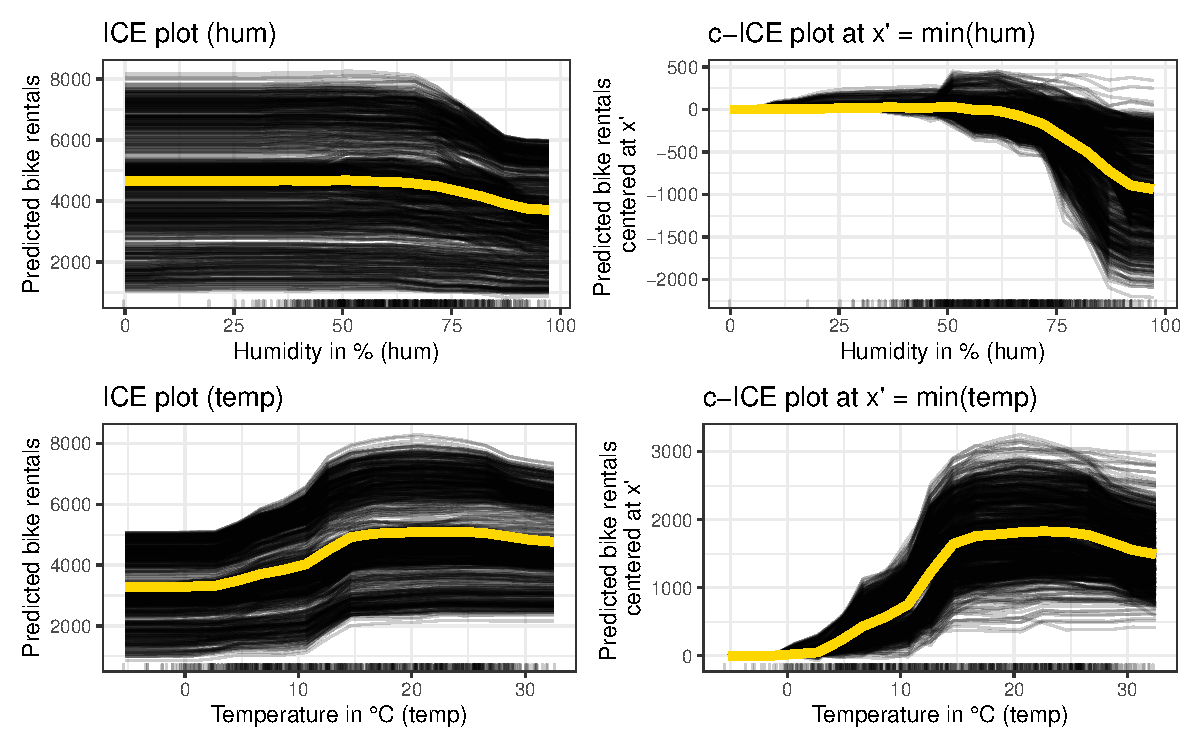
\includegraphics[width=\textwidth]{figure/cICE}
\end{center}
\end{column}
\end{columns}

%\vspace{-0.4cm}

Interpretation (yellow curve in c-ICE plot): On average, the number of bike rentals at $\sim 98$ \% humidity decreased by 1000 bikes compared to a humidity of 1 \%
\end{frame}


\begin{frame}{Centered ICE Plot (c-ICE)}

\begin{center}
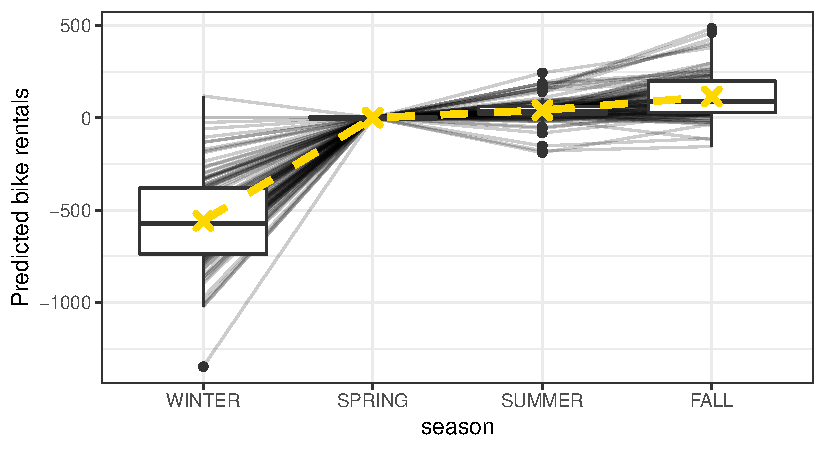
\includegraphics[width=0.6\textwidth]{figure/cICEcat}
\end{center}

\begin{itemize}
\item Centered ICE plots are useful for categorical features and can be interpreted as in LMs
\item The reference category is $x^* =$ SPRING
\item Golden crosses: Average number of bike rentals if we jump from SPRING to any other season
\end{itemize}

\end{frame}


% \frame{
% \frametitle{Derivative ICE Plot (d-ICE)}
%
% Aim: Interactions
%
% }

% \begin{frame}{Extrapolation}

% There are two sources of extrapolation:
% \lz
% \begin{enumerate}
%   \item If the model predicts in regions where it was not trained. Predictions in such regions are a bad approximation to the real underlying relationship between input and target space.
%   \lz
%   \item Averaging ICE curves at specific grid points refers to Monte Carlo integration w.r.t. a   uniform distribution and ignores how likely the data points are.
%   It might be better to integrate w.r.t. the (empirical) data distribution.
% \end{enumerate}
% \lz
% $\Rightarrow$ Biased estimates, especially in case of correlated features.
% \end{frame}

\begin{frame}{Extrapolation}

% \begin{center}
% \includegraphics[width=0.8\textwidth]{figure_man/extrapolation01.png}
% \end{center}

Extrapolation can cause issues in regions with few observations or if features are correlated
 
\begin{columns}[T]
\begin{column}{0.5\textwidth}
\centering
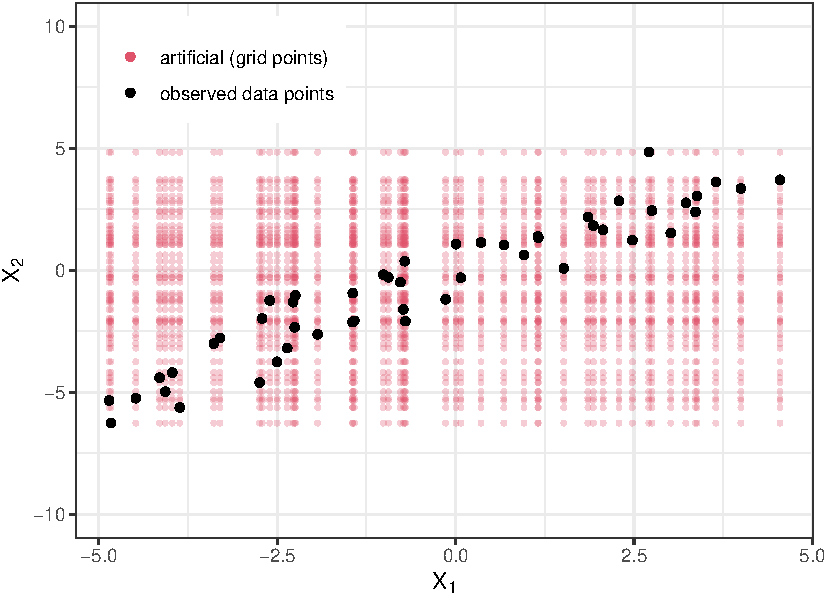
\includegraphics[width=0.8\textwidth]{figure/ale_scatter_grid}
\end{column}
\begin{column}{0.5\textwidth}
\centering
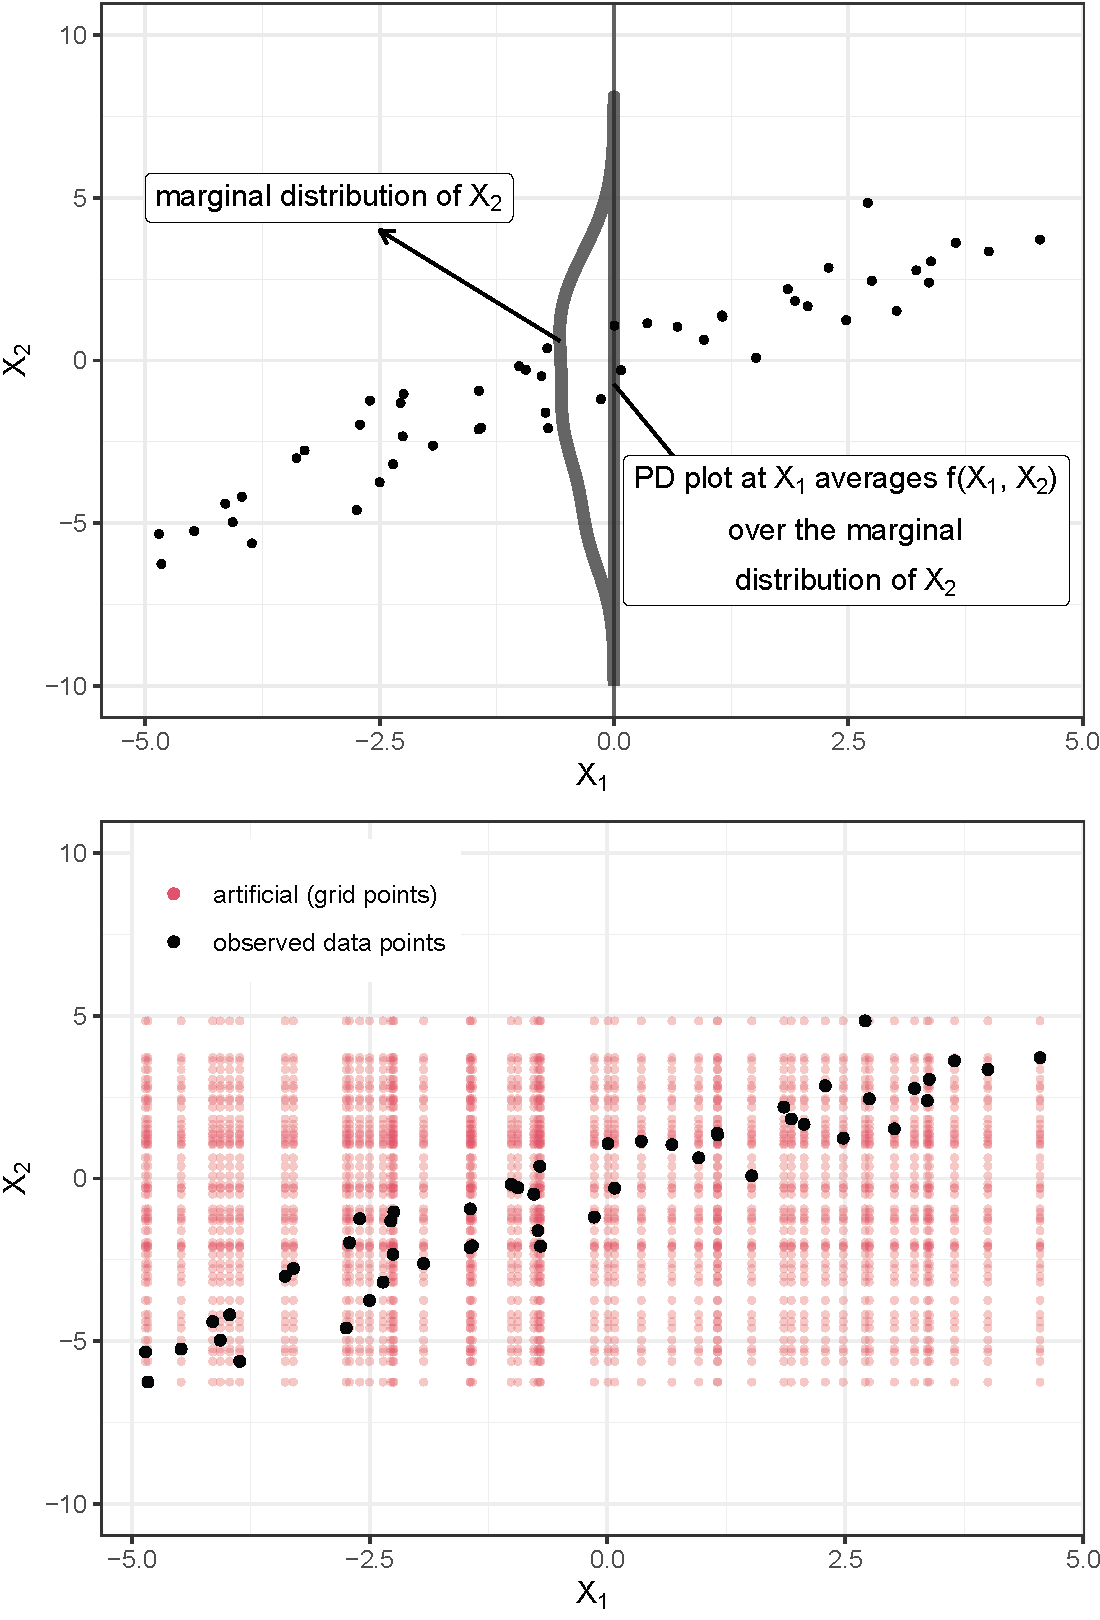
\includegraphics[width=0.8\textwidth]{figure/ale_pdplot}
\end{column}
\end{columns}

\begin{itemize}
\item \textbf{Example:} Features $x_1$ and $x_2$ are strongly correlated
\item \textbf{Black points:} Observed points of the original data
\item \textbf{\textcolor{red}{Red:}} Grid points used to calculate the ICE and PD curves (several unrealistic values)\\ %combination of feature values
$\Rightarrow$ %Unrealistic combination of feature values are used, e.g., the
PD plot at $x_1=0$ averages predictions over the whole marginal distribution of feature $x_2$\\
$\Rightarrow$ May be problematic if model behaves strange outside training distribution
%can bias ICE and PD curves Be careful with interpretations 
%\item For correlated features and in regions with few observations with care
%Extrapolation: interpret curves for highly correlated features and in feature regions with few observations with care
\end{itemize}

%
% \framebreak
%
%
% \begin{center}
% \includegraphics[width=0.8\textwidth]{figure_man/extrapolation02.png}
% \end{center}
%
% \begin{itemize}
% \item The features $x_1$ and $x_2$ are strongly correlated.
% \item \textcolor{red}{Red:} Observed points of the original data.
% \item \textcolor{green}{Green:} Grid points used to calculate the ICE and PD curves.
% \item Example: PD plot at $x_1=1.9$ averages predictions over the whole marginal distribution of feature $x_2$.
% \end{itemize}
\end{frame}




% \begin{frame}{Interactions}
%
% For PD plots, the averaging of ICE curves might \textbf{obfuscate} heterogeneous effects and interactions. \newline \(\Rightarrow\) Ideally plot ICE curves and PD plots together.
%
% \begin{center}\includegraphics[width=0.65\textwidth]{figure_man/pdp_xor.pdf} \end{center}
% %
% % \framebreak
% %
% % \begin{itemize}
% % \item
% %   For PD plots, the averaging of ICE curves might \textbf{obfuscate}
% %   heterogeneous effects and interactions. \newline \(\Rightarrow\)
% %   Ideally plot ICE curves and PD plots together.
% % \item
% %   \textbf{Extrapolation:} Interprete curves for highly correlated
% %   features and in feature regions with few observations with care.
% % \item
% %   Accumulated Local Effects (ALE) plots are a novel alternative to the PD plots developed by Apley (2020) that do not suffer from
% %   extrapolation in case of correlated features.
% % \end{itemize}
% %
% % \vspace{80pt}
% % \tiny{
% % Apley, D. W., \& Zhu, J. (2020). Visualizing the effects of predictor variables in black box supervised learning models. Journal of the Royal Statistical Society: Series B, 82(4), 1059-1086. \par}
% \end{frame}

\begin{frame}{Interactions}
\begin{itemize}
%\lz
%\item Accumulated Local Effects (ALE) plots are a novel alternative to PD plots developed by Apley (2016) that do not suffer from extrapolation in case of correlated features.

\item PD plots: averaging of ICE curves might \textbf{obfuscate} heterogeneous effects and interactions \newline \(\Rightarrow\) Ideally plot ICE curves and PD plots together

\begin{center}\includegraphics[width=0.5\textwidth]{figure/pdp_xor.pdf} \end{center}
\end{itemize}

%\footnote[frame]{Apley, Daniel W., and Jingyu Zhu (2020). Visualizing the Effects of Predictor Variables in Black Box Supervised Learning Models. Journal of the Royal Statistical Society: Series B (Statistical Methodology) 82.4: 1059-1086.}
\end{frame}


\endlecture
\end{document}
